%% 
%%	This is file 'beamer_sample.tex'
%%	according to an MPIDR's PowerPoint template (?)
%%	
%%	by Eric Naujoks
%%
%%	Problems, bugs and comments to 
%%	naujoks@demogr.mpg.de
%%

%%%%%%%%%%%%%%%%%%%%%%%%%%%%%%%%%%
%%	Praelegomena								%%
%%%%%%%%%%%%%%%%%%%%%%%%%%%%%%%%%%
%%	- Make sure that you use utf8-encoding for all your .tex-files!!! (TeXnicCenter since version 2.0)
%%	- TeXnicCenter update: MPIDR intranet > Hard- & Sortfware > Software > Script and text editors > TeXnicCenter

\documentclass[20pt]{beamer}

\usepackage[ngerman,english]{babel}
\usepackage{tikz}
\usepackage[normalem]{ulem}
\geometry{paperwidth=10in, paperheight=7.5in}
\usepackage{animate}

\usepackage[utf8]{inputenc}

\usepackage[mpidr]{./mpidr/beamerthemeMPIDR}

%% Declaring title and author
\title{A unified framework\\ of demographic time}
\subtitle{Tim Riffe \\ Jonas Sch{\"o}ley \\ Francisco Villavicencio}		%%

%%	the institute's logo
\renewcommand{\mylogo}{
\includegraphics[width=4.7in]{mpidr_logo_colour_en}}
\usepackage{color}
\definecolor{mygray}{rgb}{0.8,0.8,0.8}

\defbeamertemplate{description item}{align left}{\insertdescriptionitem\hfill}
%%	should be the very last package to be loaded
\usepackage{hyperref}

%%%%%%%%%%%%%%%%%%%%%%%%%%%%%%%%%%
%%	Beginning of the document		%%
%%%%%%%%%%%%%%%%%%%%%%%%%%%%%%%%%%
\begin{document}

%%	titlepage - fixed frame:
%%	========================

\begin{frame}
	\titlepage
\end{frame}
%-------------------
\begin{frame}
\begin{block}{objective}
We add a third dimension to the Lexis diagram to account for time-to-death. This
results in three \textit{new} kinds of 2D Lexis diagrams, and a 3D Lexis diagram
that is the intersection of the four \textit{degenerate} diagrams.
\end{block}
\color{mygray}(It turns out Lexis himself did something eerily similar, but not
identical. Happy to explain how it works too)

\end{frame}
%-------------------
\begin{frame}
\frametitle{Aspects of time we consider}
\begin{itemize}[<+->]
  \item A: chronological age
  \item P: period, calendar year
  \item C: birth cohort
  \item T: time until death
  \item D: death cohort = year of death
  \item L: ultimate complete lifespan
\end{itemize}
\end{frame}

%-------------------

\begin{frame}
\frametitle{The demographic time identity}
\vspace{-4em}
\begin{center}
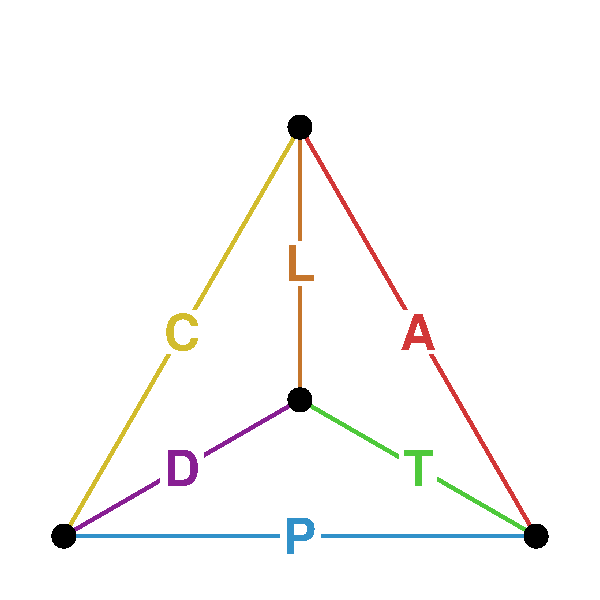
\includegraphics[scale=1.7]{Figures/TetraHedronEdgesOnly.pdf}
\end{center}
\end{frame}

%-------------------

\begin{frame}
\frametitle{APC}
\begin{center}
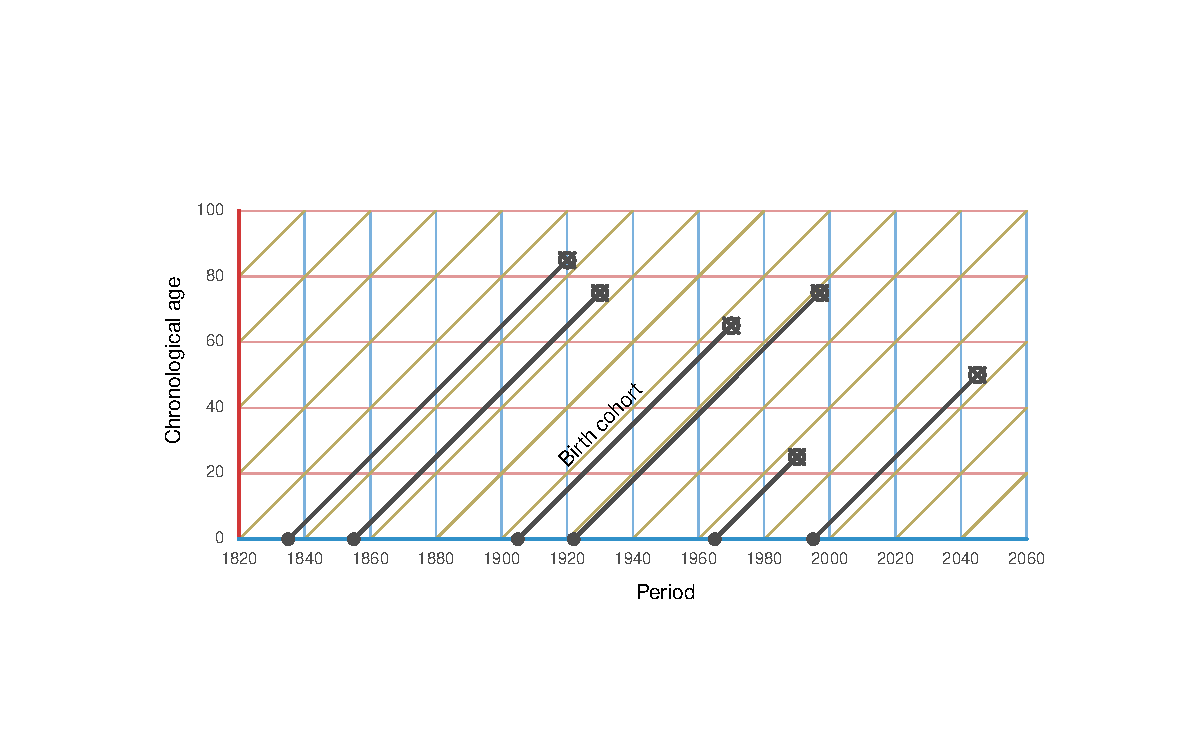
\includegraphics[trim= 200 200 200 200, scale=1.5]{Figures/APCrt.pdf}
\end{center}
\end{frame}

%-------------------

\begin{frame}
\frametitle{APC}
\begin{center}
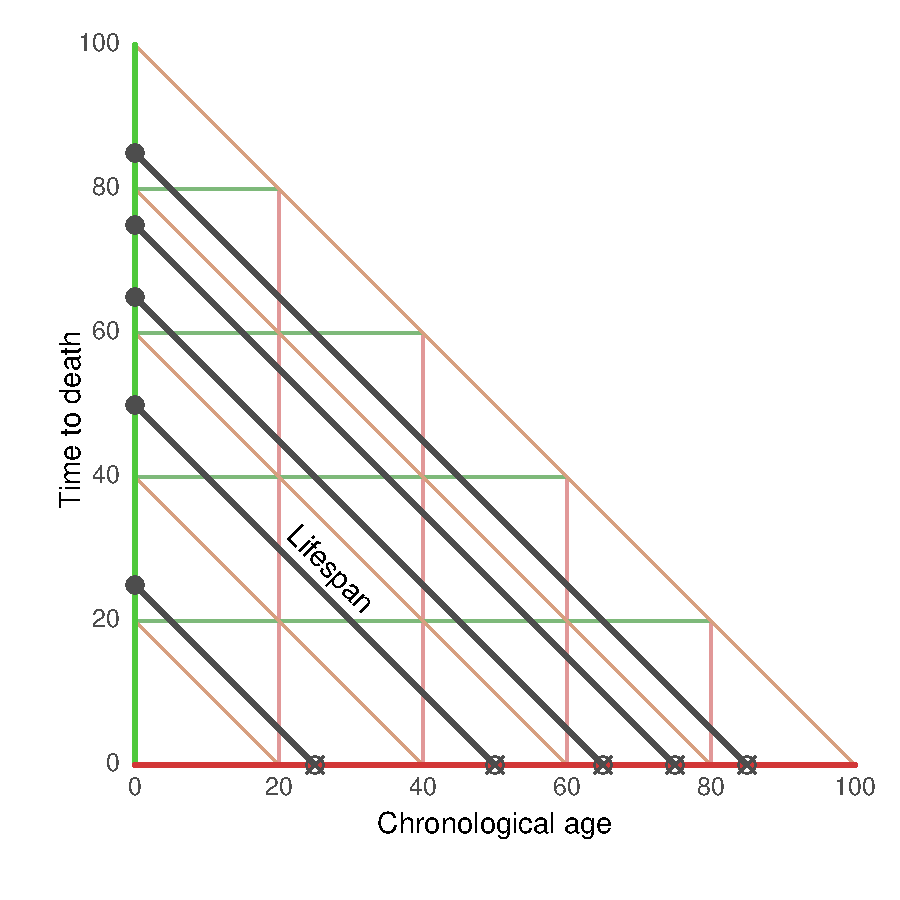
\includegraphics[ scale=1.1]{Figures/TALrt.pdf}
\end{center}
\end{frame}

%-------------------

\begin{frame}
\frametitle{The demographic time identity}
\vspace{-4em}
\begin{center}
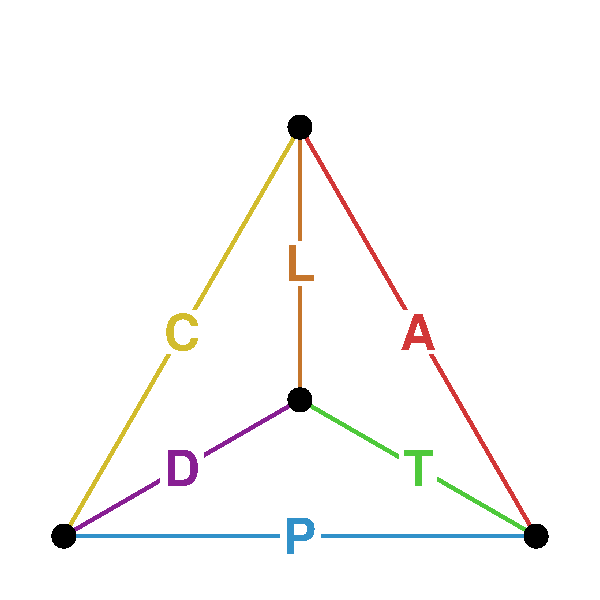
\includegraphics[scale=1.7]{Figures/TetraHedronEdgesOnly.pdf}
\end{center}
\end{frame}

%-------------------

\begin{frame}
\frametitle{The demographic time identity}
\vspace{-4em}
\begin{center}
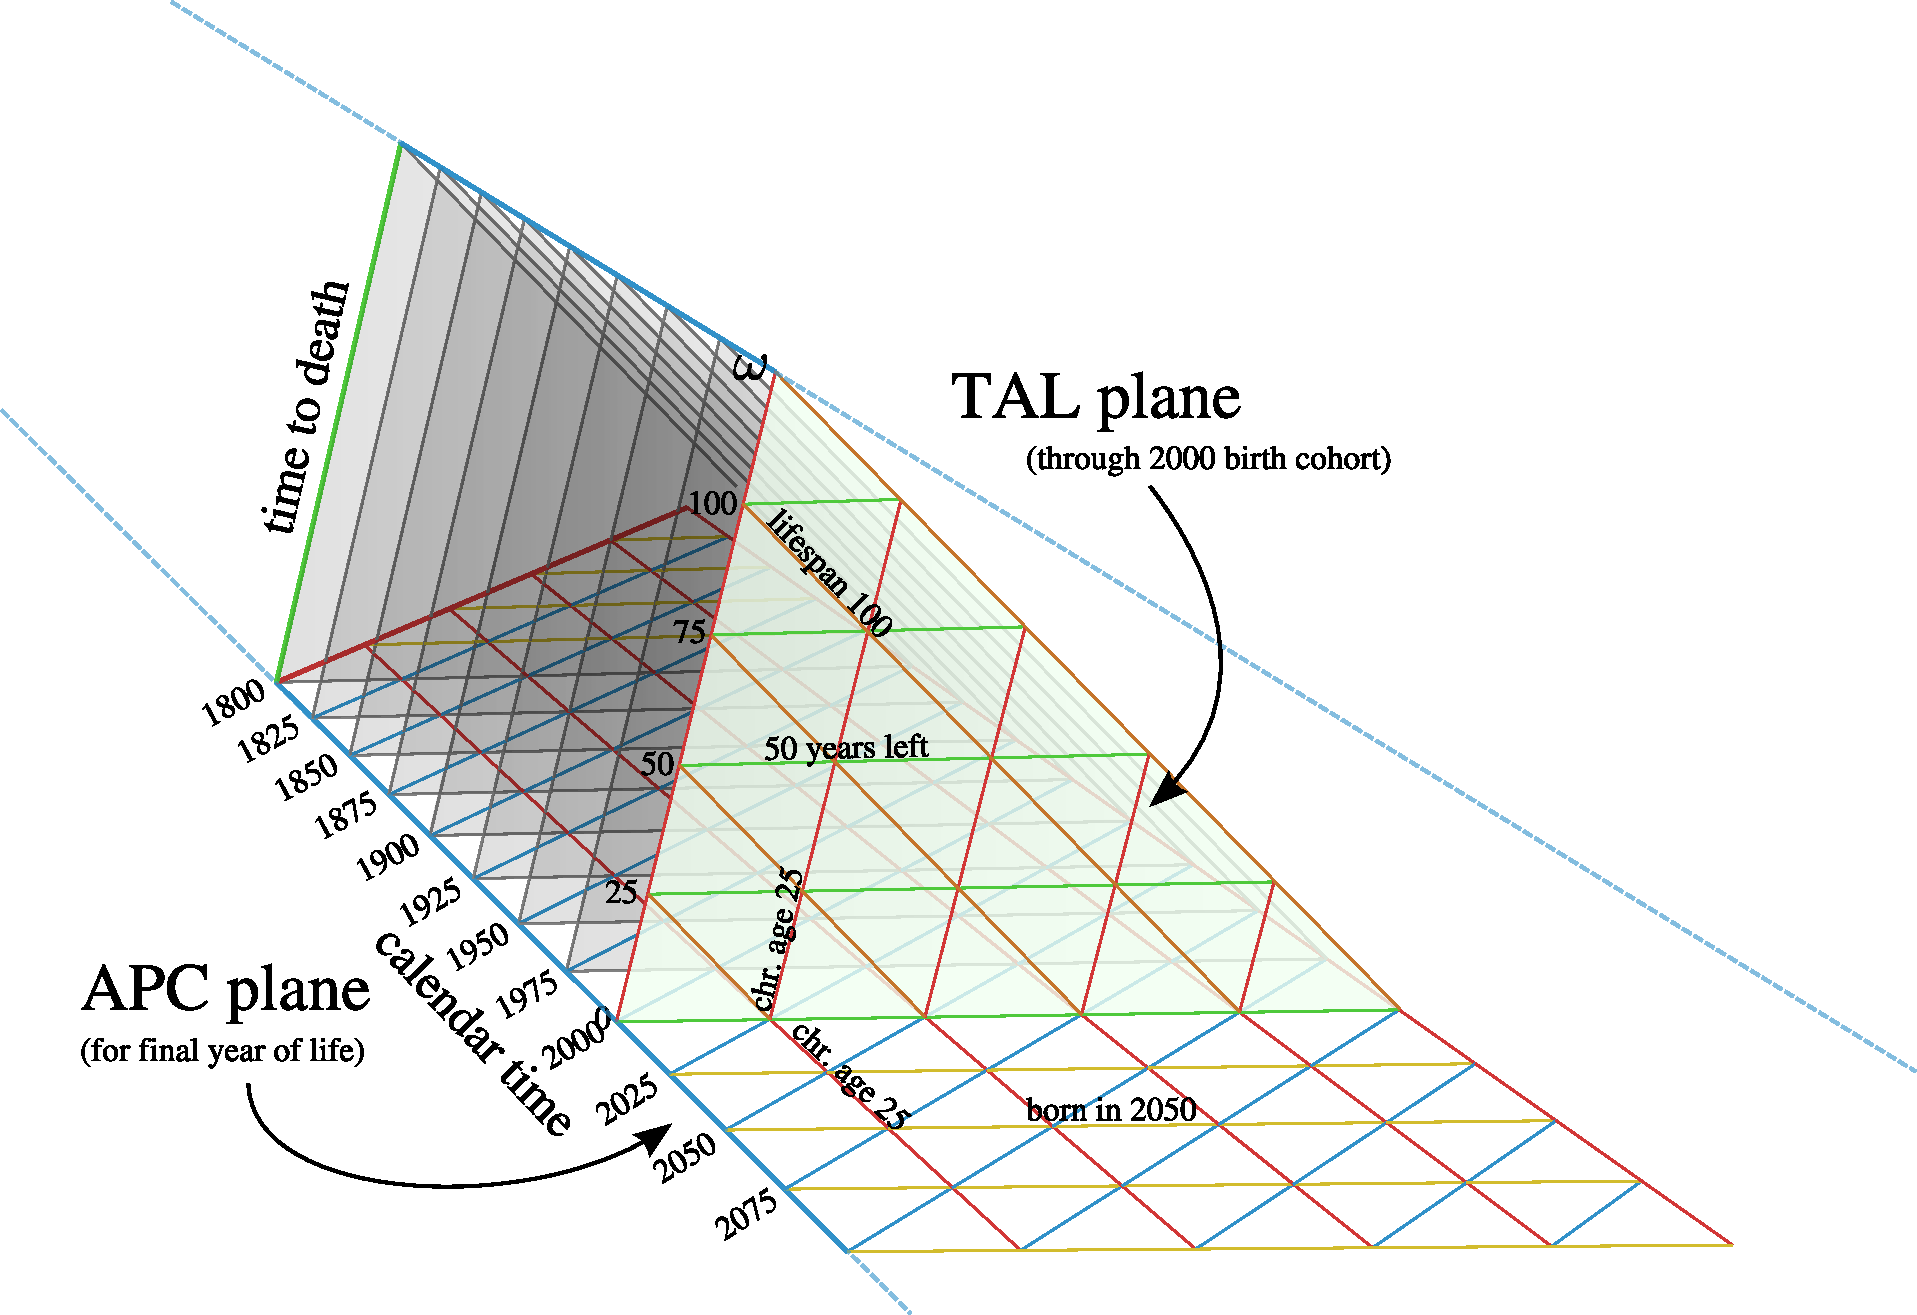
\includegraphics[scale=.8]{Figures/TALisomarkedup2PAA.pdf}
\end{center}
\end{frame}

%-------------------

\begin{frame}
\frametitle{APC can reveal patterns}
\begin{center}
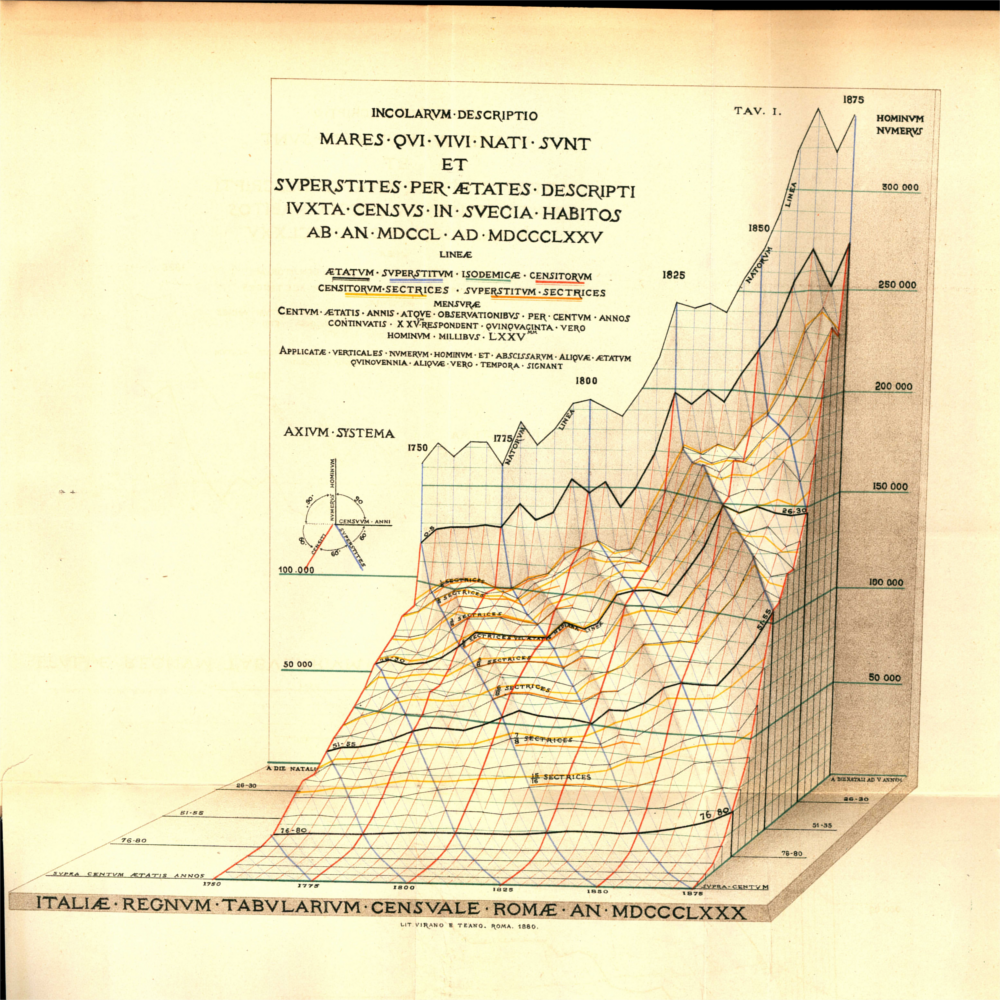
\includegraphics[trim 100 100 300
300,scale=.5]{Figures/Perozzo1000px_cropped_adj.png}
\end{center}
\end{frame}

%-------------------

\begin{frame}
\frametitle{So why more planes?}
\vspace{-4em}
\begin{center}
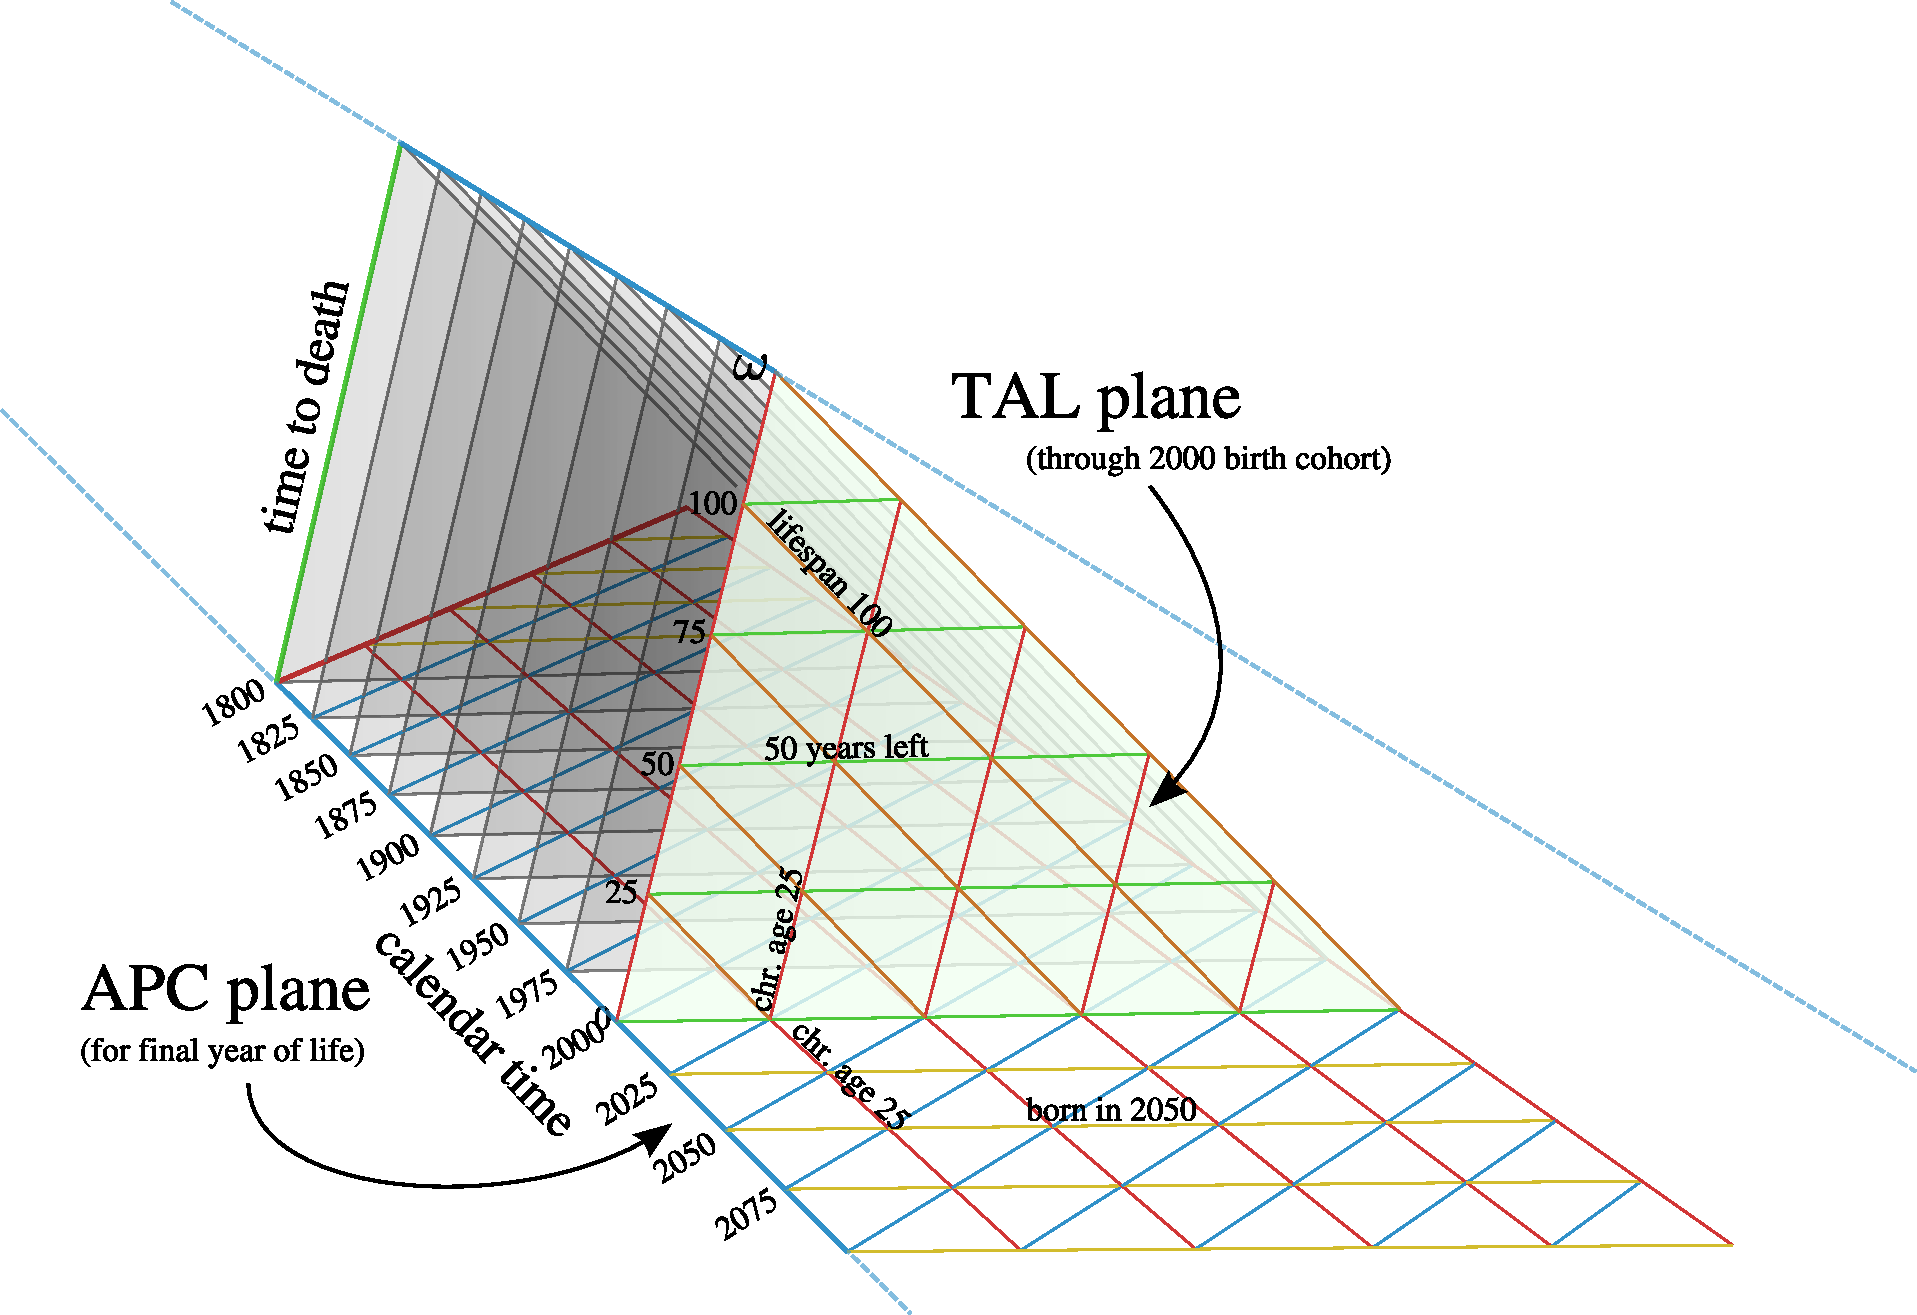
\includegraphics[scale=.8]{Figures/TALisomarkedup2PAA.pdf}
\end{center}
\end{frame}

%---------------------------

\begin{frame}
\frametitle{So why more planes?}
\normalsize
\begin{itemize}[<+->]
  \item to uncover more patterns
  \item to improve measurement
  \item to understand processes
  \item to make better models
\end{itemize}
\end{frame}

%---------------------------------

\begin{frame}
\frametitle{An example inquiry}
\normalsize
\begin{itemize}[<+->]
  \item compare end-of-life trajectories for several birth cohorts (1905 - 1925)
  \item HRS (Rand), waves 1-11 (years 1992-2012)
  \item use TAL plane to uncover patterns that APC hides
  \item this example: prevalence of poor self-reported health
\end{itemize}
\end{frame}

%---------------------------

\begin{frame}
\frametitle{1905 cohort}
\vspace{-4em}
\begin{center}
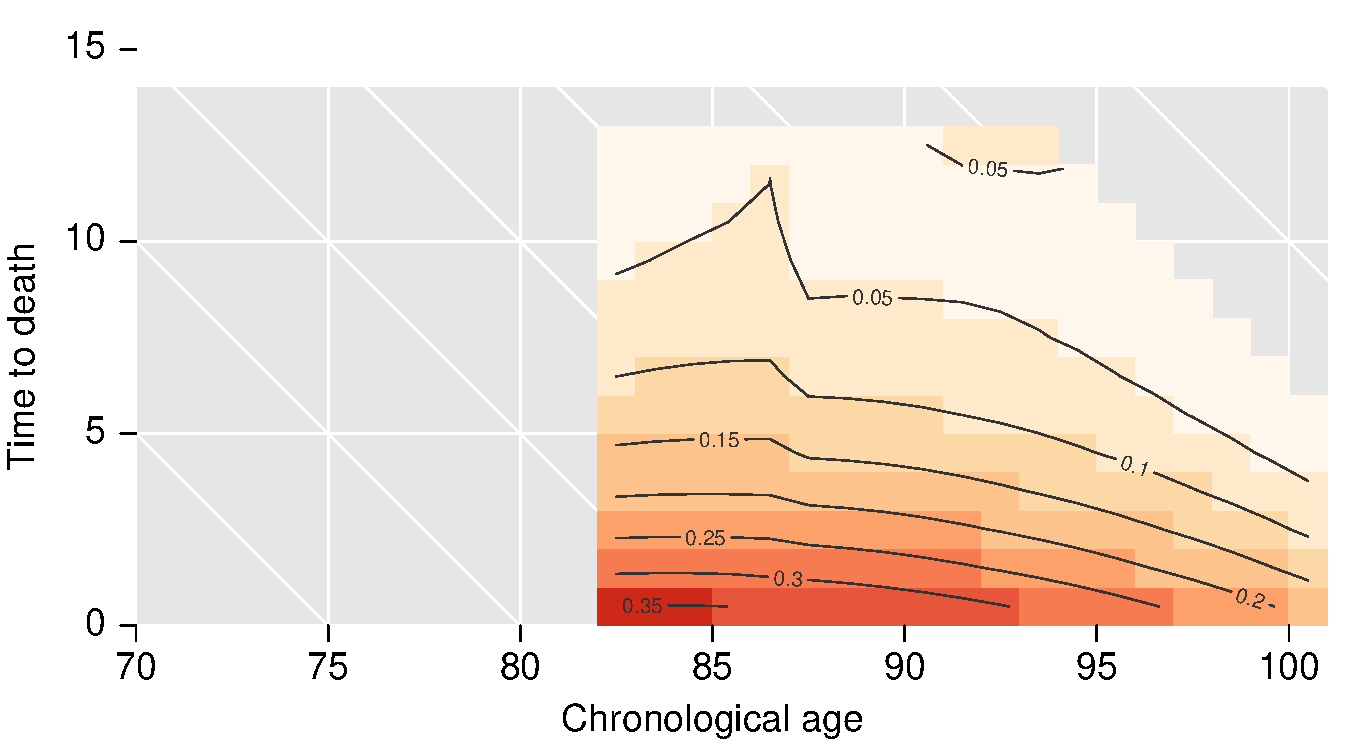
\includegraphics[scale=1]{Figures/srhpoor1905.pdf}
\end{center}
\end{frame}

%---------------------------

\begin{frame}
\frametitle{1910 cohort, looking pretty similar}
\vspace{-4em}
\begin{center}
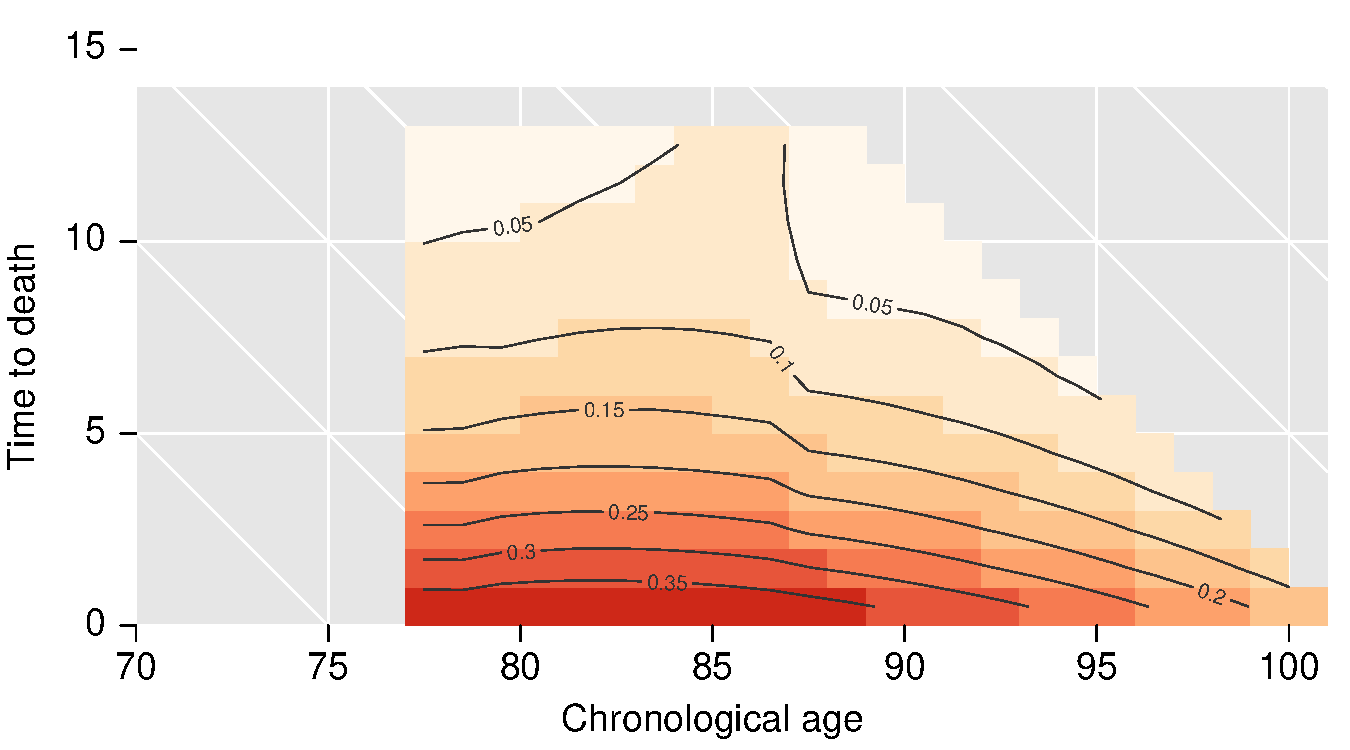
\includegraphics[scale=1]{Figures/srhpoor1910.pdf}
\end{center}
\end{frame}

%---------------------------

\begin{frame}
\frametitle{1915 cohort, looking pretty similar}
\vspace{-4em}
\begin{center}
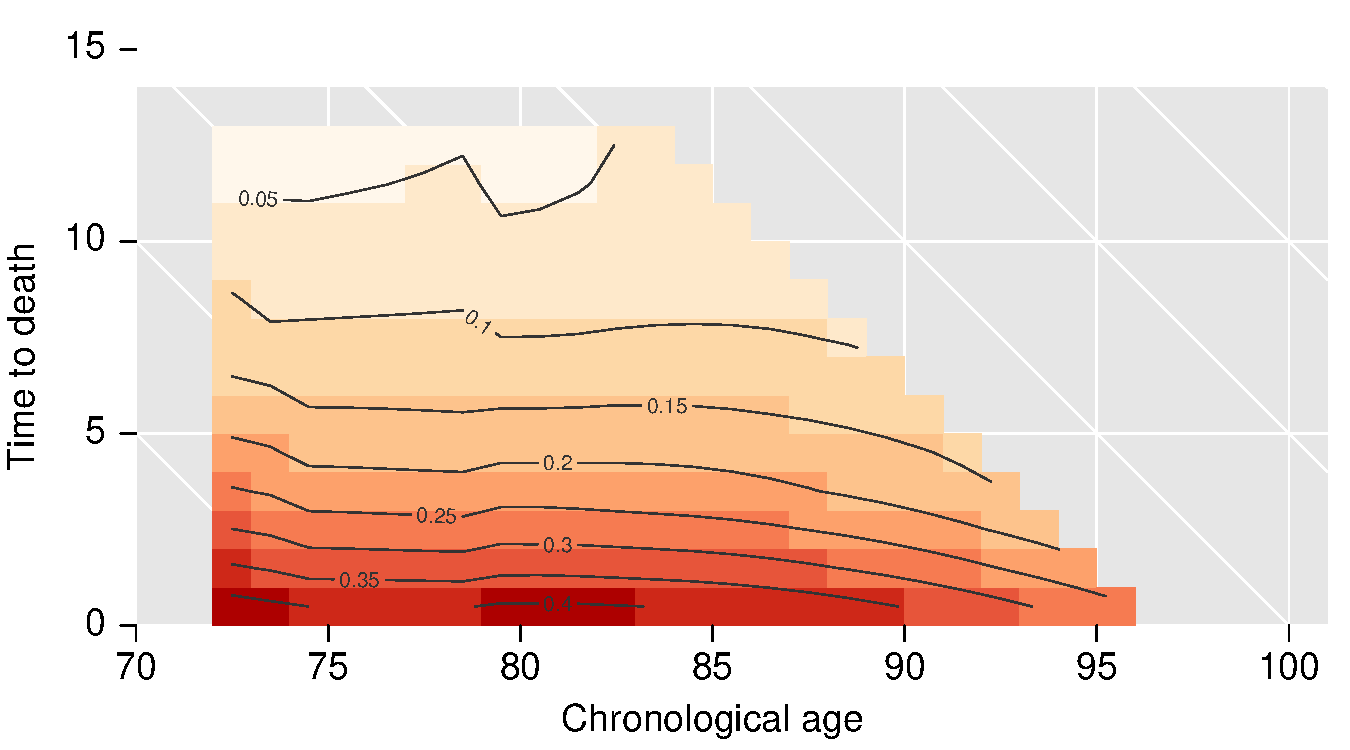
\includegraphics[scale=1]{Figures/srhpoor1915.pdf}
\end{center}
\end{frame}

%---------------------------

\begin{frame}
\frametitle{1920 cohort, looking pretty similar}
\vspace{-4em}
\begin{center}
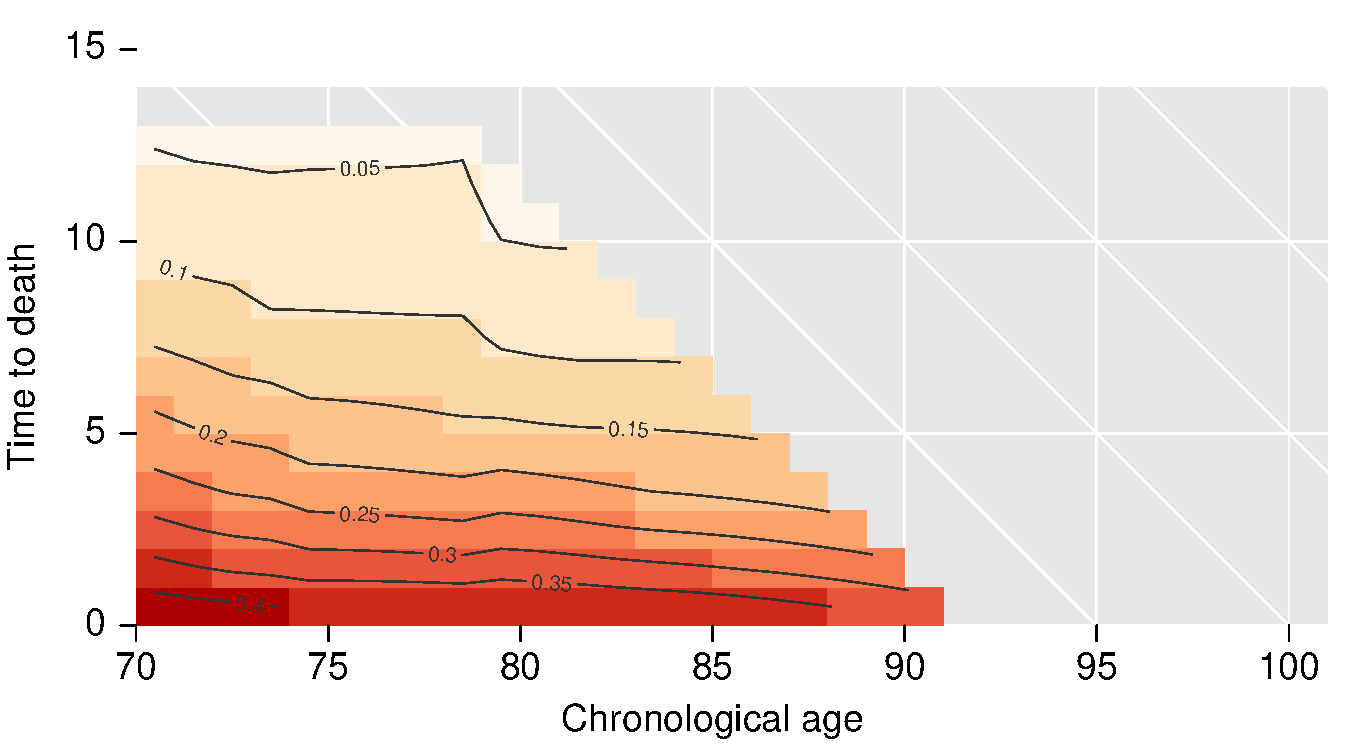
\includegraphics[scale=1]{Figures/srhpoor1920.pdf}
\end{center}
\end{frame}

%---------------------------

\begin{frame}
\frametitle{1925 cohort, looking pretty similar}
\vspace{-4em}
\begin{center}
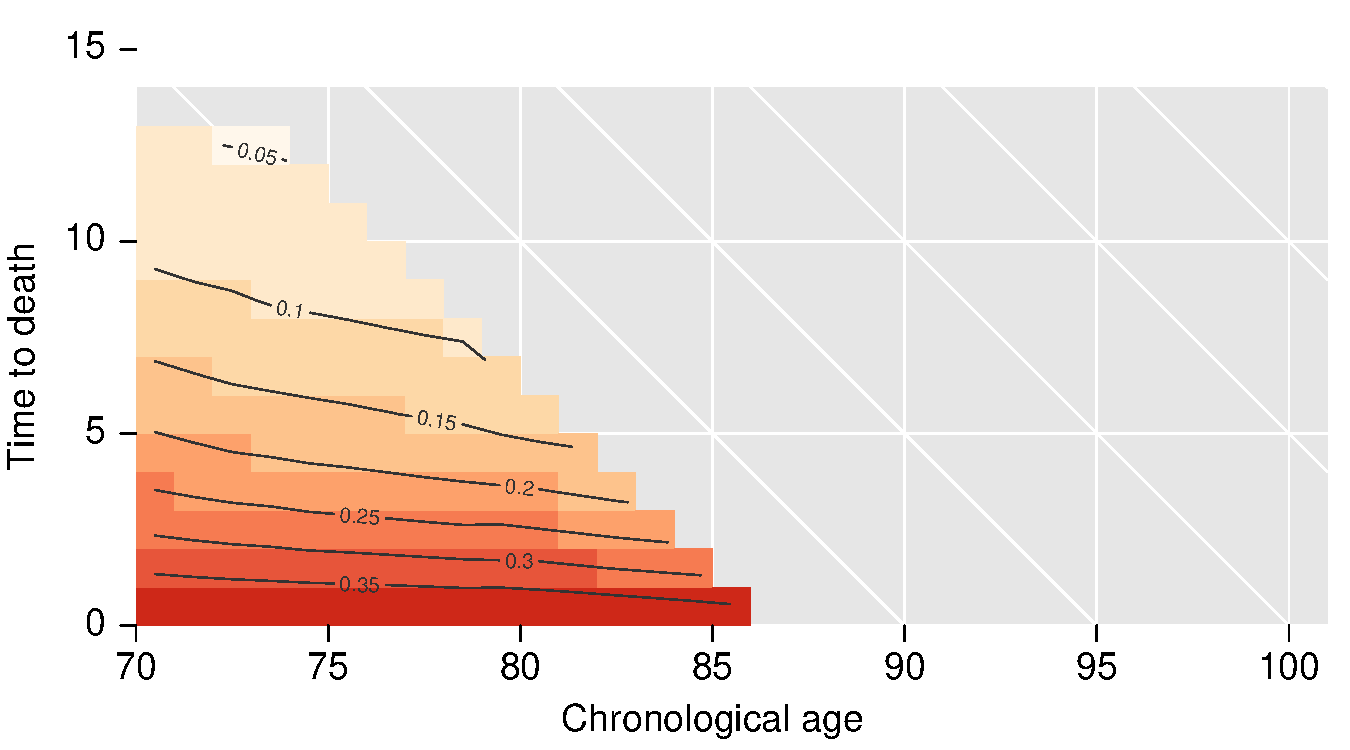
\includegraphics[scale=1]{Figures/srhpoor1925.pdf}
\end{center}
\end{frame}

%----------------------------------

\begin{frame}
\frametitle{So why more planes?}
\normalsize
\begin{itemize}[<+->]
  \item easier to detect patterns
  \item to better understand the relationships between the measures of
  demographic time
\end{itemize}
\end{frame}

%----------------------------------

\begin{frame}
\frametitle{You should}
\normalsize
\begin{itemize}[<+->]
  \item make an origami tetrahedron and label its edges with the demographic
  time measures
  \item visualize data structured in this way ASAP, because you might see new
  and exciting things
\end{itemize}
\end{frame}

%----------------------------------

\begin{frame}
\frametitle{Thanks!}
\vspace{-4em}
\begin{center}
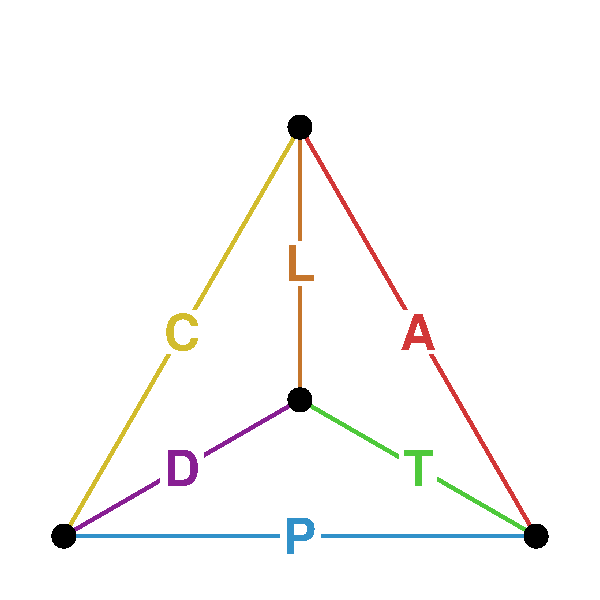
\includegraphics[scale=1.7]{Figures/TetraHedronEdgesOnly.pdf}
\end{center}
\end{frame}

%%%%%%%%%%%%%%%%%%%%%%%%%%%%%%%%%%
%%	End of the document			%%
%%%%%%%%%%%%%%%%%%%%%%%%%%%%%%%%%%
\end{document}










